\documentclass{standalone}
\usepackage{xstring}
\usepackage{tikz}
\usetikzlibrary{calc, decorations.pathreplacing, calligraphy}
\usepackage{xifthen}
\usepackage{amsmath}
\usetikzlibrary{bayesnet}

\newcommand{\Height}{0.8cm}% Adjust size of square as desired
\newcommand{\Width}{1.6cm}% Adjust size of square as desired

\tikzset{GreySquare/.style={
    inner sep=0pt,
    text width=\Width,
    minimum size=\Height,
    draw=black,
    fill=black!20,
    align=center
    }
}
\tikzset{LightGreySquare/.style={
    inner sep=0pt,
    text width=\Width,
    minimum size=\Height,
    draw=black,
    fill=black!5,
    align=center
    }
}

\tikzset{GreenSquare/.style={
    inner sep=0pt,
    text width=\Width,
    minimum size=\Height,
    draw=black,
    fill=green!15,
    align=center
    }
}
\tikzset{DarkGreenSquare/.style={
    inner sep=0pt,
    text width=\Width,
    minimum size=\Height,
    draw=black,
    fill=green!50,
    align=center
    }
}
\tikzset{RedSquare/.style={
    inner sep=0pt,
    text width=\Width,
    minimum size=\Height,
    draw=black,
    fill=red!15,
    align=center
    }
}
\tikzset{DarkRedSquare/.style={
    inner sep=0pt,
    text width=\Width,
    minimum size=\Height,
    draw=black,
    fill=red!50,
    align=center
    }
}
\tikzset{BlueSquare/.style={
    inner sep=0pt,
    text width=\Width,
    minimum size=\Height,
    draw=black,
    fill=blue!15,
    align=center
    }
}
\tikzset{DarkBlueSquare/.style={
    inner sep=0pt,
    text width=\Width,
    minimum size=\Height,
    draw=black,
    fill=blue!50,
    align=center
    }
}
\tikzset{Red2Square/.style={
    inner sep=0pt,
    text width=\Width,
    minimum size=\Height,
    draw=black,
    fill=orange!25,
    align=center
    }
}
\tikzset{DarkRed2Square/.style={
    inner sep=0pt,
    text width=\Width,
    minimum size=\Height,
    draw=black,
    fill=orange!80,
    align=center
    }
}
\tikzset{Blue2Square/.style={
    inner sep=0pt,
    text width=\Width,
    minimum size=\Height,
    draw=black,
    fill=yellow!25,
    align=center
    }
}
\tikzset{DarkBlue2Square/.style={
    inner sep=0pt,
    text width=\Width,
    minimum size=\Height,
    draw=black,
    fill=yellow!70,
    align=center
    }
}
\tikzset{Square/.style={
    inner sep=0pt,
    text width=\Width,
    minimum size=\Height,
    draw=black,
    fill=red!0,
    align=center
    }
}

\begin{document}

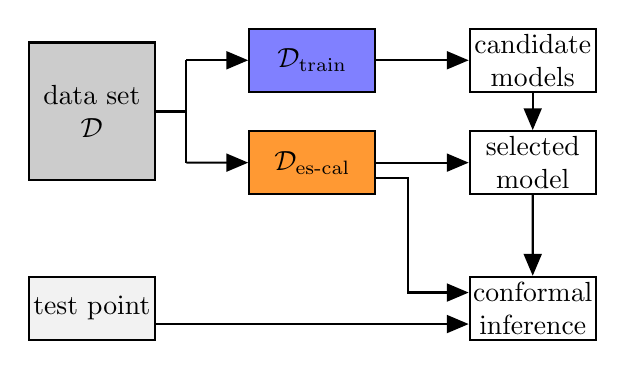
\begin{tikzpicture}[draw=black, thick, x=\Width,y=\Height]
    
    \node (D)[GreySquare, minimum height = 1.75cm] at (0,2.5) {data set \\ $\mathcal{D}$};
    
    \node (Dtrain) [DarkBlueSquare, right of=D, xshift=1.8cm, yshift=0.65cm] {$\mathcal{D}_{\text{train}}$};
 
    \node (models) [Square, right of=Dtrain, xshift=1.8cm, yshift=0cm] {candidate models};
  
    \node (Dcal) [DarkRed2Square, below of=Dtrain, yshift=-0.3cm] {$\mathcal{D}_{\text{es-cal}}$};

    \node (BestModel) [Square, right of=Dcal, xshift=1.8cm, yshift=0cm] {selected model};
     
    \coordinate [right of=D, xshift=0.2cm] (s1);
        \draw (D.east) -- (s1);
    \coordinate [above of=s1, yshift=-0.35cm] (s2);
    \coordinate [below of=s1, yshift=0.35cm] (s3);
        \draw (s1) -- (s3);
        \draw (s1) -- (s2);
        \draw [->] (s2) -- (Dtrain.west);
        \draw [->] (s3) -- (Dcal.west);
    
    
   \node (Dtest) [LightGreySquare, below of=D, yshift=-1.5cm] {test point};

   \node (CI) [Square, right of=Dtest, xshift=4.6cm, yshift=0cm] {conformal inference};
 

   \coordinate [right of=Dcal, xshift=0.3cm] (s4);
%   \draw[->] (s4) |- (CI);
   \draw[->] ($(Dcal.east)+(0,-0.25)$) -- ($(Dcal.east)+(0.25,-0.25)$) |- ($(CI.west)+(-0.25,0.25)$) -- ($(CI.west)+(0,0.25)$);
   \draw[->] ($(Dtest.east)+(0,-0.25)$) -- ($(CI.west)+(0,-0.25)$);

   \draw[->] (BestModel.south) -- (CI);

   \draw[->] (models.south) -- (BestModel.north);
   \draw[->] (Dcal.east) -- (BestModel.west);

   \draw[->] (Dtrain.east) -- (models.west);

   % \draw[->] (Dtest.south) -- ($(Dtest.south)+(0,-0.25)$) -| ($(BestModel.east)+(0.25,0)$) -- (BestModel.east);


    % \coordinate [right of=Dcal, xshift=0.3cm] (s4);
    % \coordinate [right of=Dtest, xshift=0.3cm] (s5);
    %     \draw (Dcal) -- (s4);
    %     \draw (Dtest) -- (s5);
    % \coordinate [below of=s4, yshift=0.3cm] (s6);
    %     \draw (s4) -- (s5);
    
%    \node (es) [GreenSquare, minimum height = 1.75cm, right of=s6, xshift=0.6cm]
%    {conformal\\ES};
%        \draw [->] (s6) -- (es.west);
        
    
    
\end{tikzpicture}


\end{document}

%%% Local Variables:
%%% mode: latex
%%% TeX-master: t
%%% End:
